\documentclass[tikz,border=3pt]{standalone}
\usepackage[utf8]{inputenc}
\usepackage[T1]{fontenc}
\usepackage{lmodern}
\renewcommand{\familydefault}{\sfdefault}
\usepackage{sansmath}\sansmath
\usepackage{chemfig}
\usepackage{pgfplots}\pgfplotsset{compat=1.18,/pgf/number format/use comma,/pgf/number format/1000 sep={.}}
\usetikzlibrary{arrows.meta,calc,positioning,decorations.pathmorphing,patterns}
% paleta del sitio
\definecolor{nar}{HTML}{E8680C}\definecolor{narc}{HTML}{FFB35C}\definecolor{hielo}{HTML}{FFF3E8}
\definecolor{tinta}{HTML}{1D1D1F}\definecolor{gris}{HTML}{6E6E73}\definecolor{lila}{HTML}{7C5CF0}
\definecolor{azul}{HTML}{2F6FD6}\definecolor{menta}{HTML}{17A673}\definecolor{coral}{HTML}{E8342A}
\begin{document}
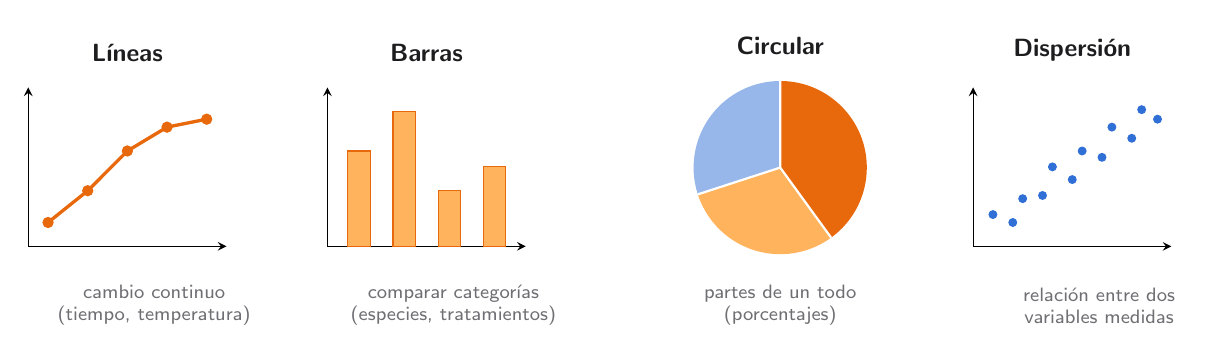
\begin{tikzpicture}[font=\small]
\pgfplotsset{mini/.style={width=4.1cm,height=3.6cm,axis lines=left,xtick=\empty,ytick=\empty,title style={font=\small\bfseries,text=tinta}}}
\begin{axis}[mini,title={Líneas},at={(0,0)},xmin=0,xmax=10,ymin=0,ymax=10]
\addplot[nar,very thick,mark=*,mark options={scale=0.7,fill=nar}] coordinates {(1,1.5)(3,3.5)(5,6)(7,7.5)(9,8)};
\end{axis}
\begin{axis}[mini,title={Barras},at={(3.8cm,0)},ybar,bar width=8pt,xmin=0.3,xmax=4.7,ymin=0,ymax=10]
\addplot[fill=narc,draw=nar] coordinates {(1,6)(2,8.5)(3,3.5)(4,5)};
\end{axis}
\begin{scope}[shift={(9.55cm,1.0cm)}]
\node[font=\small\bfseries,text=tinta] at (0,1.55) {Circular};
\fill[nar] (0,0) -- (90:1.1) arc (90:-54:1.1) -- cycle;
\fill[narc] (0,0) -- (-54:1.1) arc (-54:-162:1.1) -- cycle;
\fill[azul!50] (0,0) -- (-162:1.1) arc (-162:-270:1.1) -- cycle;
\draw[white,thick] (0,0) -- (90:1.1) (0,0) -- (-54:1.1) (0,0) -- (-162:1.1);
\end{scope}
\begin{axis}[mini,title={Dispersión},at={(12.0cm,0)},xmin=0,xmax=10,ymin=0,ymax=10]
\addplot[only marks,mark=*,azul,mark options={fill=azul,scale=0.7}] coordinates {(1,2)(2,1.5)(2.5,3)(3.5,3.2)(4,5)(5,4.2)(5.5,6)(6.5,5.6)(7,7.5)(8,6.8)(8.5,8.6)(9.3,8)};
\end{axis}
\node[font=\scriptsize,text=gris,align=center] at (1.6,-0.75) {cambio continuo\\(tiempo, temperatura)};
\node[font=\scriptsize,text=gris,align=center] at (5.4,-0.75) {comparar categorías\\(especies, tratamientos)};
\node[font=\scriptsize,text=gris,align=center] at (9.55,-0.75) {partes de un todo\\(porcentajes)};
\node[font=\scriptsize,text=gris,align=center] at (13.6,-0.75) {relación entre dos\\variables medidas};
\end{tikzpicture}
\end{document}
